\section{交叉引用与文献}
\label{sec:00-crossref}

\subsection{为什么不要手打编号}

"第 4 章""图 3.2""式 (2)"这类编号，如果手打，章节一调整就全对不上。
统一做法是：先在对象旁边写标签，再用 \verb|\cref| 引用，编号自动生成。

写法：

\begin{lstlisting}[language=TeX]
\section{图片}
\label{sec:00-pictures}              % 节的标签

\begin{figure}[htbp]
  \centering
  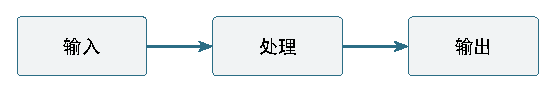
\includegraphics[width=.7\linewidth]{figures/05-pictures/demo-flow}
  \caption{数据流示意}
  \label{fig:00-flow}                % 图的标签
\end{figure}

引用时写成：见\cref{sec:00-pictures}、见\cref{fig:00-flow}。
\end{lstlisting}

效果：见\cref{sec:00-pictures}、见\cref{fig:00-flow}。表格、公式、代码清单
也一样：\cref{tab:00-compare}、\cref{eq:00-speedup}、\cref{lst:00-bubble}。
章节也可以引用，例如\cref{ch:00-guide}。

标签命名沿用"类型:章-节-序号"：\texttt{ch:} 章、\texttt{sec:} 节、
\texttt{fig:} 图、\texttt{tab:} 表、\texttt{eq:} 公式、\texttt{lst:} 代码。
标签名只用英文、数字和短横线，不要用中文和空格。

\subsection{参考文献}

引用别人的书或论文分两步：先在\textbf{本章}的 \texttt{refs.bib} 里登记条目，
再在正文里引用。

写法：

\begin{lstlisting}[language=TeX]
流水线的基本概念见经典教材\citep{patterson2020}；
\citet{amdahl1967} 很早就指出串行部分会限制整体加速比；
指令集规范这类文档同样登记成条目再引用\citep{riscvspec}。
\end{lstlisting}

效果：流水线的基本概念见经典教材 \citep{patterson2020}；
\citet{amdahl1967} 很早就指出串行部分会限制整体加速比；
指令集规范这类文档同样登记成条目再引用 \citep{riscvspec}。

\verb|\citep| 把出处放进括号，\verb|\citet| 把作者当句子成分，两种按语境挑一种。
条目本身的写法：

\begin{lstlisting}[language=TeX]
@book{patterson2020,
  author    = {Patterson, David A. and Hennessy, John L.},
  title     = {Computer Organization and Design},
  edition   = {RISC-V},
  publisher = {Morgan Kaufmann},
  year      = {2020},
}
\end{lstlisting}

三条纪律：

\begin{enumerate}
  \item 条目加在\textbf{自己章}的 \texttt{refs.bib} 里，不要去改别的章的文件；
  \item \textbf{引用键在全書范围内必须唯一}。同一本书被两章引用时，只在其中一章登记，
        另一章直接写同一个键即可——上面引用的 \texttt{patterson2020} 就登记在第 1 章，
        本章直接引用它。重复登记会让编译直接失败（BibTeX 报 \texttt{Repeated entry}）；
  \item 书末的参考文献表由各章 \texttt{refs.bib} 自动汇总，不用手工维护；
  \item 图书要写版次，网页和规范类要注明访问日期。
\end{enumerate}
